% Created 2023-03-30 Thu 19:40
% Intended LaTeX compiler: pdflatex
\documentclass{article}
    \usepackage{blindtext}
    \usepackage{geometry}
    \geometry{
      a4paper,
      total={166mm,227mm},
      left=22mm,
      top=30mm,
      }
    \usepackage[utf8]{inputenc}
    \usepackage[T1]{fontenc}
    \usepackage{fixltx2e}
    \usepackage{graphicx}
    \usepackage{longtable}
    \usepackage{float}
    \usepackage{wrapfig}
    \usepackage{rotating}
    \usepackage[normalem]{ulem}
    \usepackage{amsmath}
    \usepackage{textcomp}
    \usepackage{marvosym}
    \usepackage{wasysym}
    \usepackage{amssymb}
    \usepackage{hyperref}
    \usepackage{mathpazo}
    \usepackage{color}
    \usepackage{enumerate}

    \definecolor{bg}{rgb}{0.95,0.95,0.95}
    \definecolor{bg1}{rgb}{0.9,0.9,0.9}
    \tolerance=1000
                    \usepackage{listings}
\usepackage{xcolor}
\lstset{language=Python,backgroundcolor=\color{black!5}, basicstyle=\footnotesize\ttfamily, columns=fullflexible, breaklines, frame= tb}

    \linespread{1.1}
    \hypersetup{pdfborder=0 0 0}
\author{Ved Rudani Vijay Panchal}
\date{\today}
\title{Frequency Generator using OpAmp}
\hypersetup{
 pdfauthor={Ved Rudani Vijay Panchal},
 pdftitle={Frequency Generator using OpAmp},
 pdfkeywords={},
 pdfsubject={},
 pdfcreator={Emacs 27.1 (Org mode 9.3)}, 
 pdflang={English}}
\begin{document}

\maketitle
\tableofcontents

\pagebreak

\begin{center}
\Large
\textbf{Function Generator using OpAmp}


\vspace{0.9cm}
\normalsize
\textbf{Ved Rudani}


\textbf{Vijay Panchal}


\vspace{1.5cm}


\colorbox{bg1}{
\begin{minipage}{1\textwidth}\centering
        \vspace{1.5cm}
        \Large
        \textbf{Abstract}

        \begin{minipage}{0.7\textwidth}
        \vspace{.8cm}
        \normalsize
        Function generator are useful tools in academia and industries. Mostly they are avalaible in market. In this project we are trying to understand and study simple frequency generators with use of OpAmp. We usec generic OpAmp Ic LM741, which is single package and easy to understand with benefit of extensive acedemic experince.
        \vspace{1.5cm}
        \end{minipage}

\end{minipage}}

\vspace{1.5cm}
\noindent
\color{grey} \rule{\linewidth}{0.5mm}
\end{center}



\section{Introduction}
\label{sec:org78ed879}
Function generator is circuit which generates periodic function with predictable frequencies with respect to time. Here, we will study only mono frequency generator but it can also generate superposed functions. Signals from Function generator comes in many forms but mostly it is either sinusoidal or square wave. We will generate sinusoidal, square and triangle wave as output. 

We used basic circuits with few modification as our need. With use of IC LM741 we used OpAmp in our circuit. 

For Sinusoidal wave we used Wein Bridge circuit, which is easy to understand and impliment. Also, wein bridge circuit is quite less noice compare to it's compitition RC phase shift Oscillator, which have more component than Wein bridge and more complicated to understand. For Square wave we used standard astable multivibrator cicuit, with little modification. Lastly, Triangle wave can be made from just attaching Integrator to our square wave output with some regulation.

Now, each circuit ( this wave form generator) has different block, basically we divided whole circuit in there block. Main work for us is to combine all of this. We wandered across CMOS families, BJTs but finally we sattled into physical swith which is coupled for power transmission and also for output change.

\section{Blocks}
\label{sec:orgaa23a61}


As told in introduction each circuit is in their blocks. First block for sine wave which is nothing but wien bridge circuit, second is sqaure which is astable multivibrator, third for triangular wave which integrator attached to second block (square wave block).


\begin{figure}[htbp]
\centering
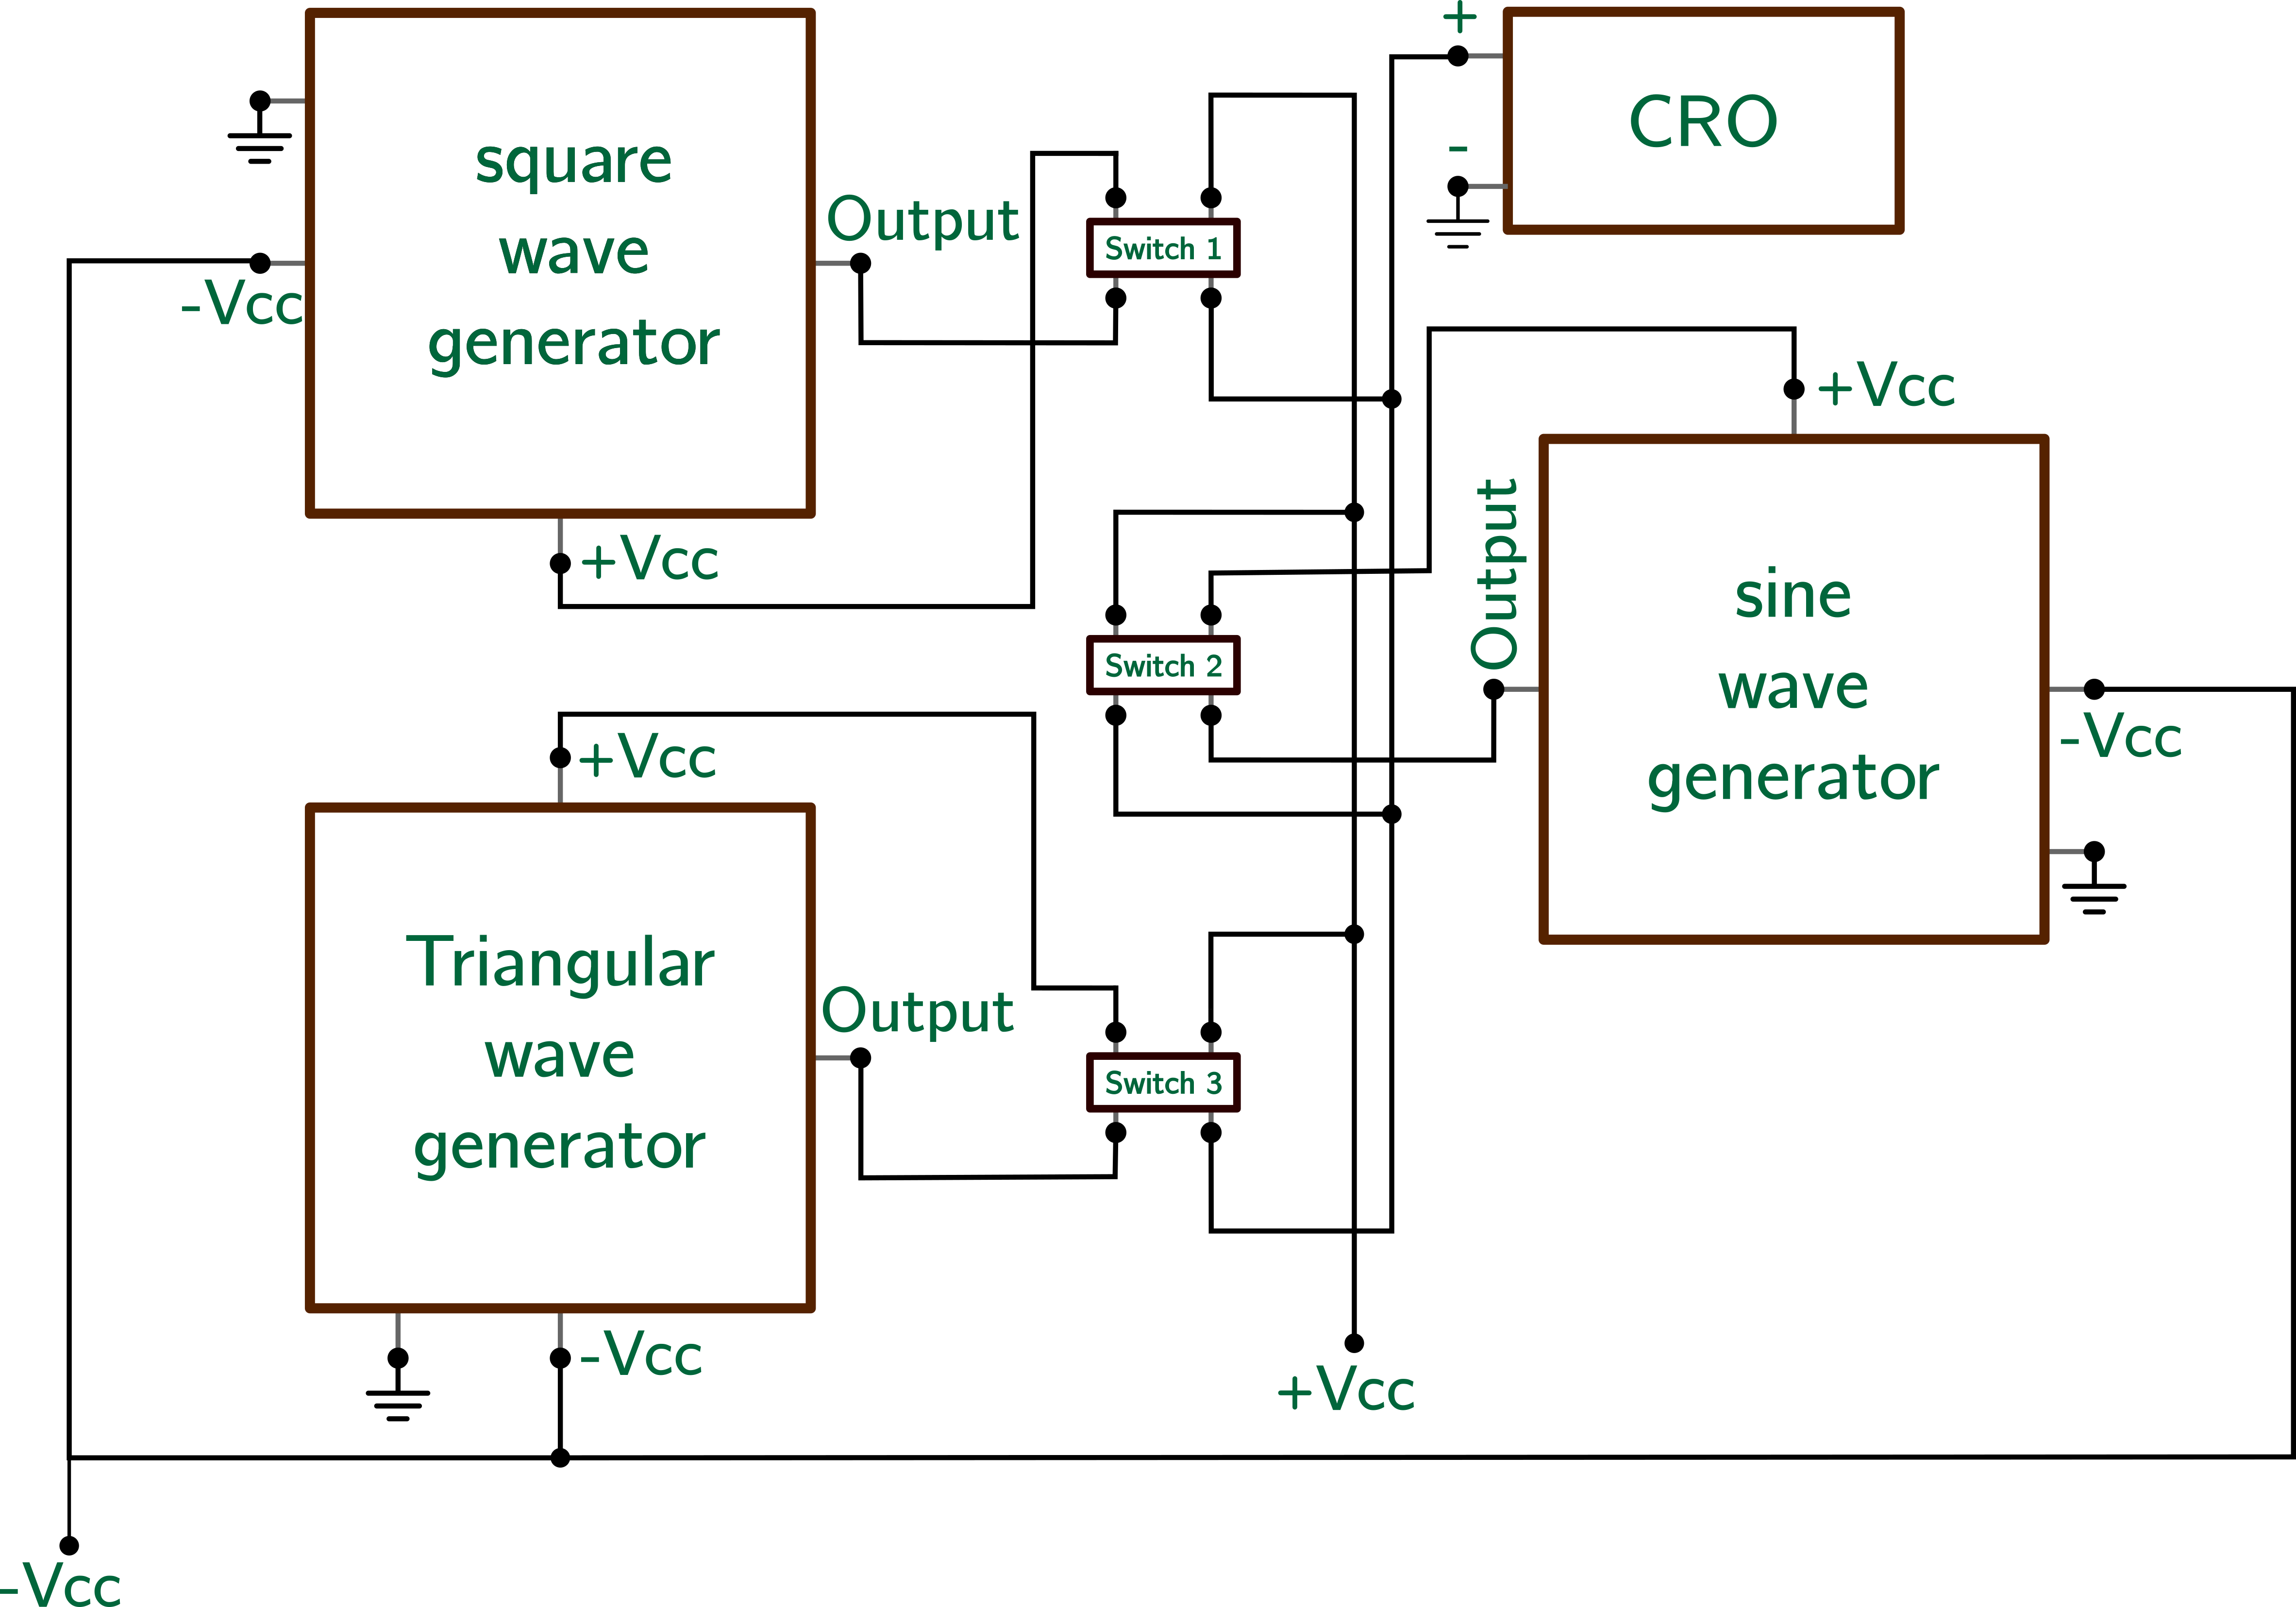
\includegraphics[width=.95\textwidth]{imgs/blocks.png}
\caption{\label{fig:org8486585}Block diagram of our function generator}
\end{figure}


\subsection{Block 1: Sine wave generator}
\label{sec:orga76e445}


In first block, we have basic circuit of wein bridge. You can see in figure 1. In center we have OpAmp (IC LM741). This is amplifier with RC component attached with input and output. Here, at one end there is RC parallel component and at other end series RC component. 

\begin{figure}[htbp]
\centering
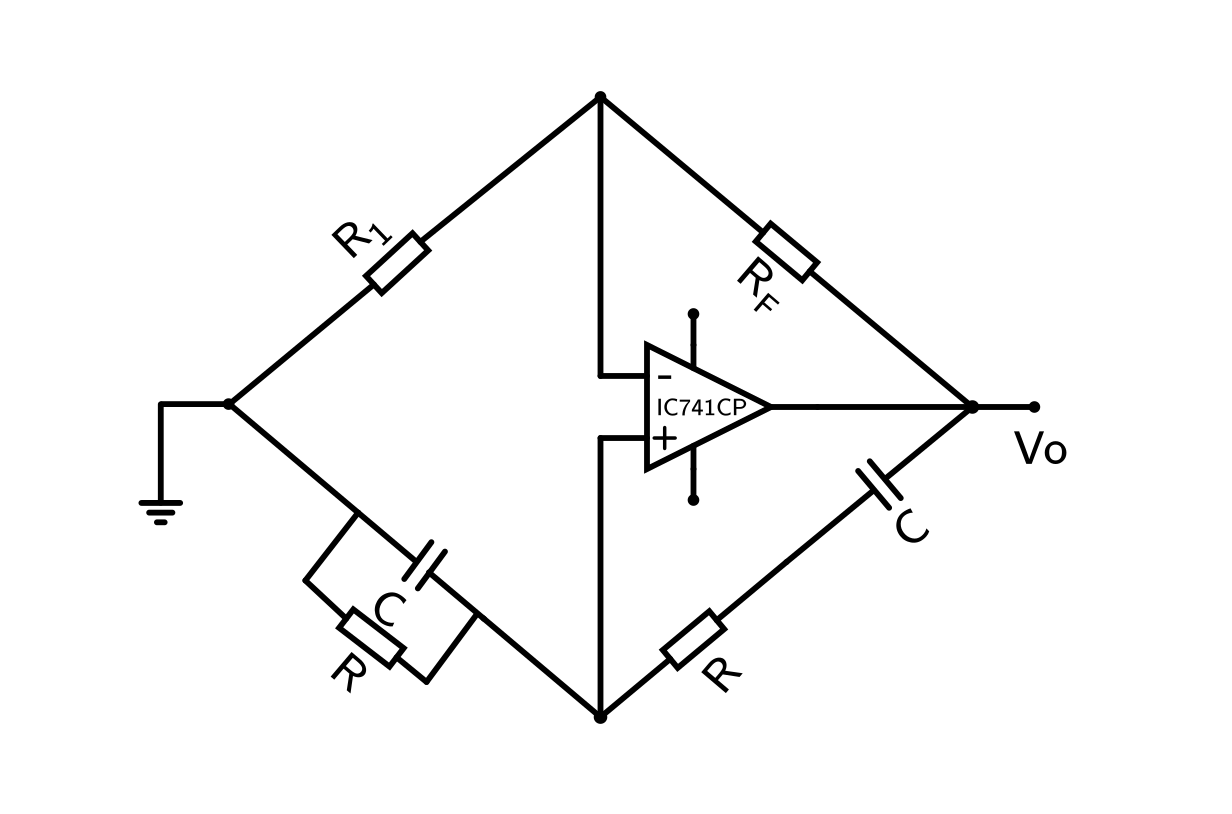
\includegraphics[width=.7\textwidth]{imgs/sine.png}
\caption{\label{fig:orgd972286}Wein bridge circuit}
\end{figure}

Here, frequency is given by, 

\begin{equation}
\label{eq:orgb803ed2}
  f =\frac{1}{2 \pi RC}
\end{equation}

For sustaing oscilation gain must be 3 and for non inverting amplifier gain, 

\begin{equation}
\label{eq:orgb4bae7a}
  A = 1+\frac{R_{F}}{R_{1}} = 3
\end{equation}

So, we get relation \(R_{F}=R_{1}\)


\begin{figure}[htbp]
\centering
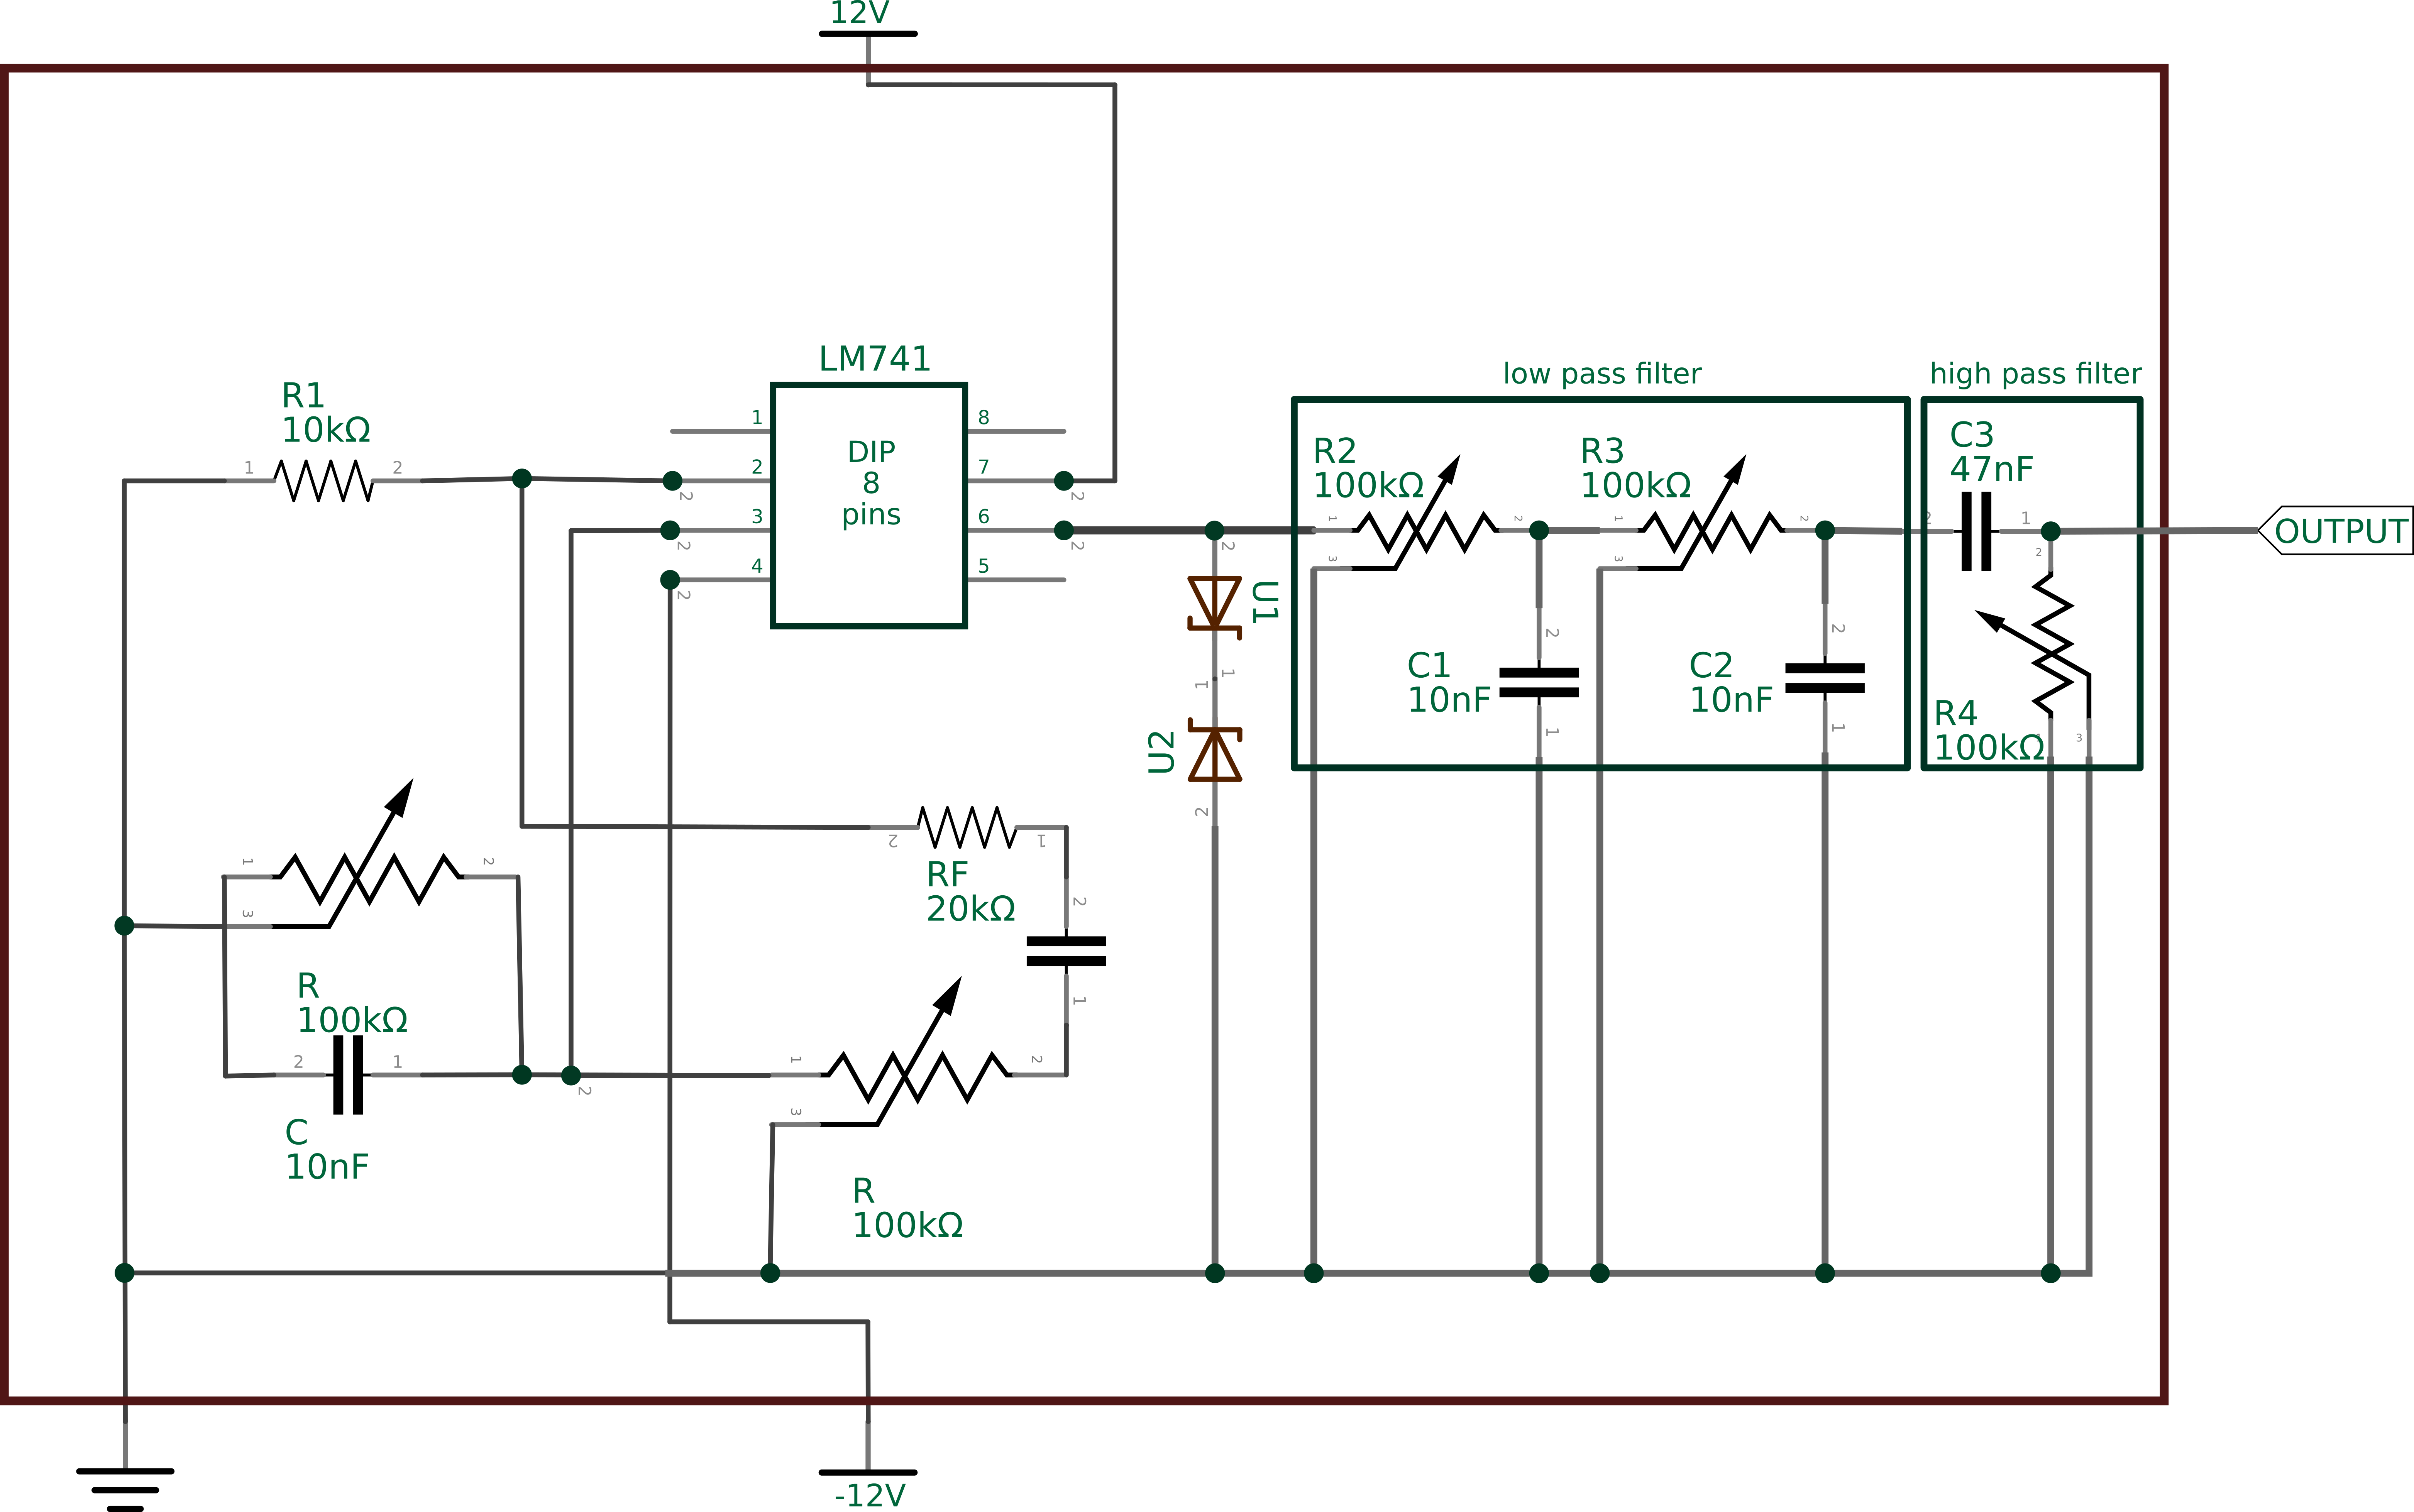
\includegraphics[width=0.95 \textwidth]{imgs/sinereal.png}
\caption{\label{fig:org22ba6e0}Our block 1, which consinst of IC741CP}
\end{figure}


Here, you can see our block circuit, at the end we attached two zener diode for regulation to the output. As you can see OpAmp in IC LM741 package. Power supply given from  4 and 7 to 12V and -12V. We chose \(R_{1}=12k\Omega\). By relation of \(R_{1}\) and \(R_{F}\), we got \(R_{F}=24k\Omega\).

For frequency range we used Potential with max range of \(100k\Omega\). So, lowest and maximum frequency whould be (with constant capacitance at \(50nF\)),

\begin{equation*}
\label{eq:org42211f7}
  f_{min} = \frac{1}{2\pi\times100k\times 10n} \approx 159 hz
\end{equation*}

\begin{equation*}
\label{eq:orgc1296c7}
  f_{max} = \frac{1}{2\pi\times100\times 10n} \approx 159k hz
\end{equation*}

So, frequency range would be \(159 hz\) to \(159k hz\)


\subsection{Block 2: Square wave generator}
\label{sec:org0b9a3e3}

As square wave generator we have basic astable multivibrator. This circuit works on scenario where output will have to stable state and it will swing between them, hence the name. When circuit is \(+V_{sat}\), we will have high signal output and when circuit is \(-V_{sat}\), we will have low signal output. So, we will have square wave as desired. The circuit for astable multivibrator is shown below.

\begin{figure}[htbp]
\centering
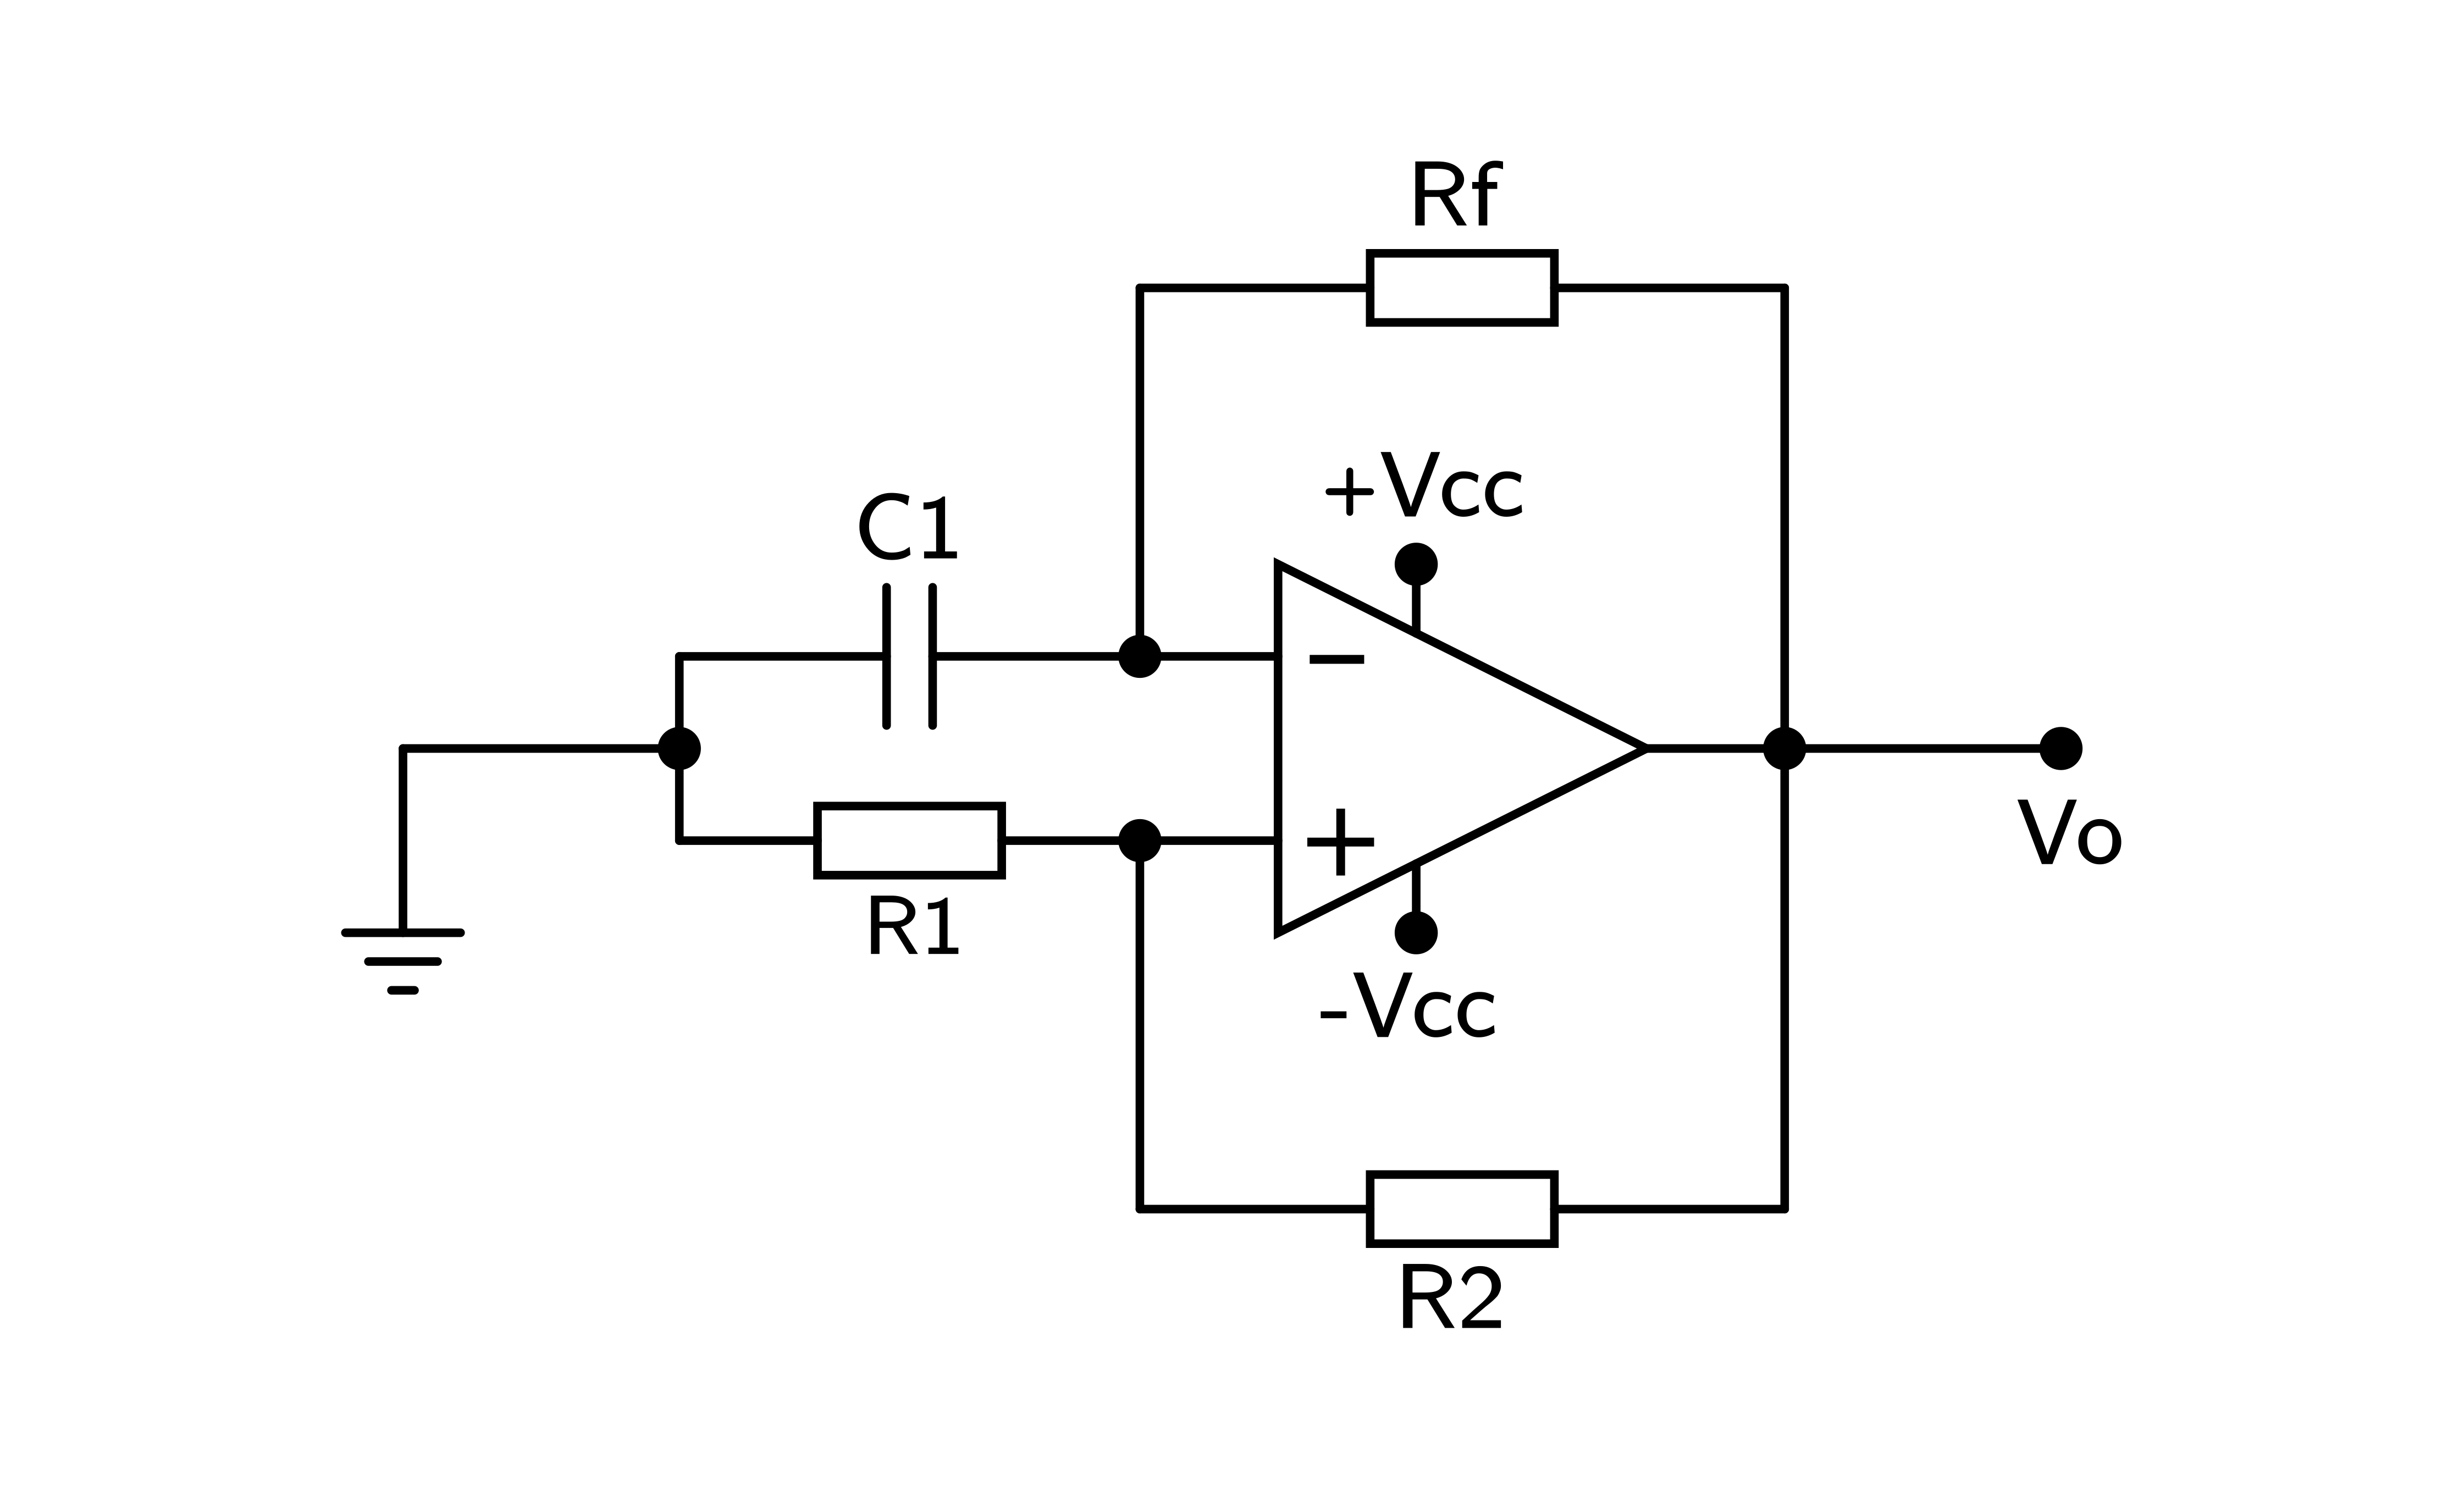
\includegraphics[width=0.7 \textwidth]{imgs/square.png}
\caption{\label{fig:org26c3f2e}astable multivibrator circuit}
\end{figure}

Here, frequency would be, 

\begin{equation}
\label{eq:orgcdc5051}
  f =\frac{1}{2 RC ln(\frac{2R_{1}+R_{2}}{R_{2}})}
\end{equation}

If, we take \(R_{2}=1.16R_{1}\) then, 

\begin{equation}
\label{eq:org2f007fe}
  f =\frac{1}{2RC}
\end{equation}

\begin{figure}[htbp]
\centering
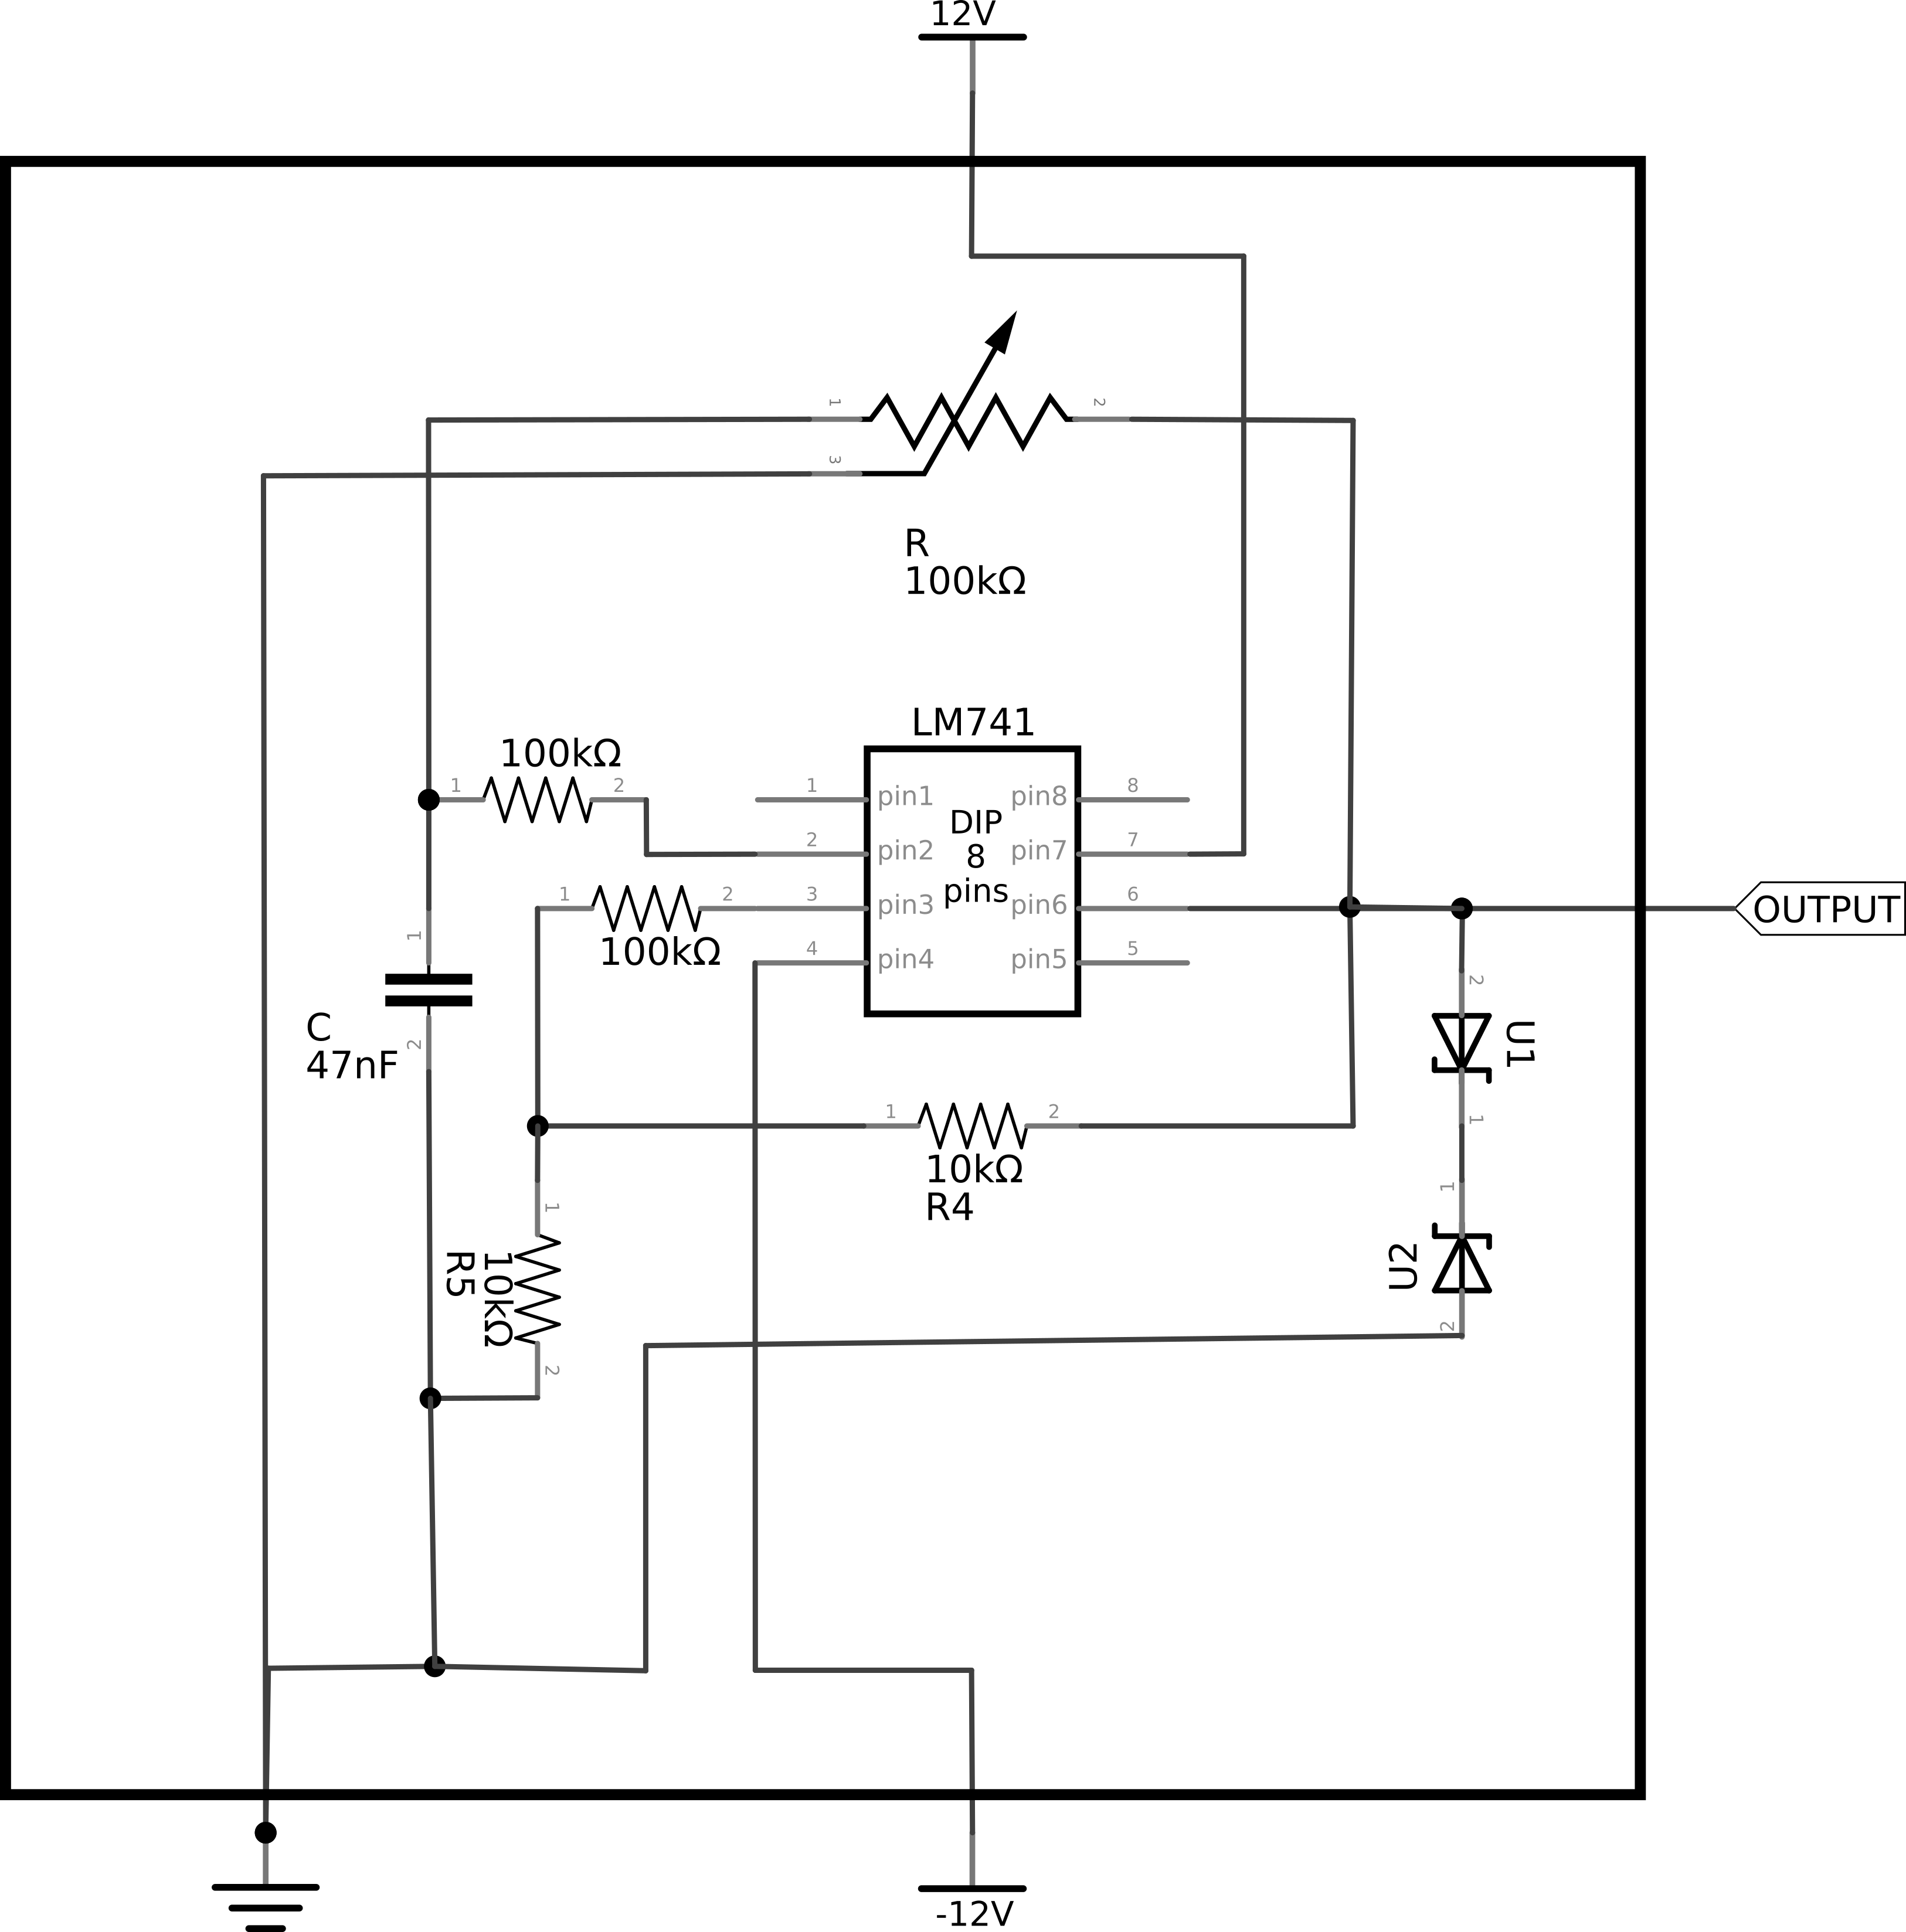
\includegraphics[width=0.95 \textwidth]{imgs/squarereal.png}
\caption{\label{fig:org3bf3901}second block: square wave generator}
\end{figure}

Here, we took \(R_{1} = 10k\Omega\) and \(R_{2} = 11.6k\Omega\) such that \(\frac{R_{2}}{R_{1}}=1.16\). Also, you can see that we employed \(100k\Omega\) in input terminals for accurate and reliable signal.

Frequency range would be of (for constant capacitance at \(50nF\)),

\begin{equation*}
\label{eq:orgaa994ed}
  f_{min} =\frac{1}{2\times 100k\times 50n} \approx 100 hz
\end{equation*}

\begin{equation*}
\label{eq:org3470ed3}
  f_{max} =\frac{1}{2\times 100 \times 50n} \approx 100 khz
\end{equation*}


\subsection{Block 3: Triangluar Wave generator}
\label{sec:org85c5923}

We basically extend block 2 with integrator circuit. Which would give triangular wave as intended. Here, this integrator circuit differs from basic circuit that \(100k\Omega\) as feedback resister is joined. Which would give better stability and accurate output. Circuit diagram is shown below,



\begin{figure}[htbp]
\centering
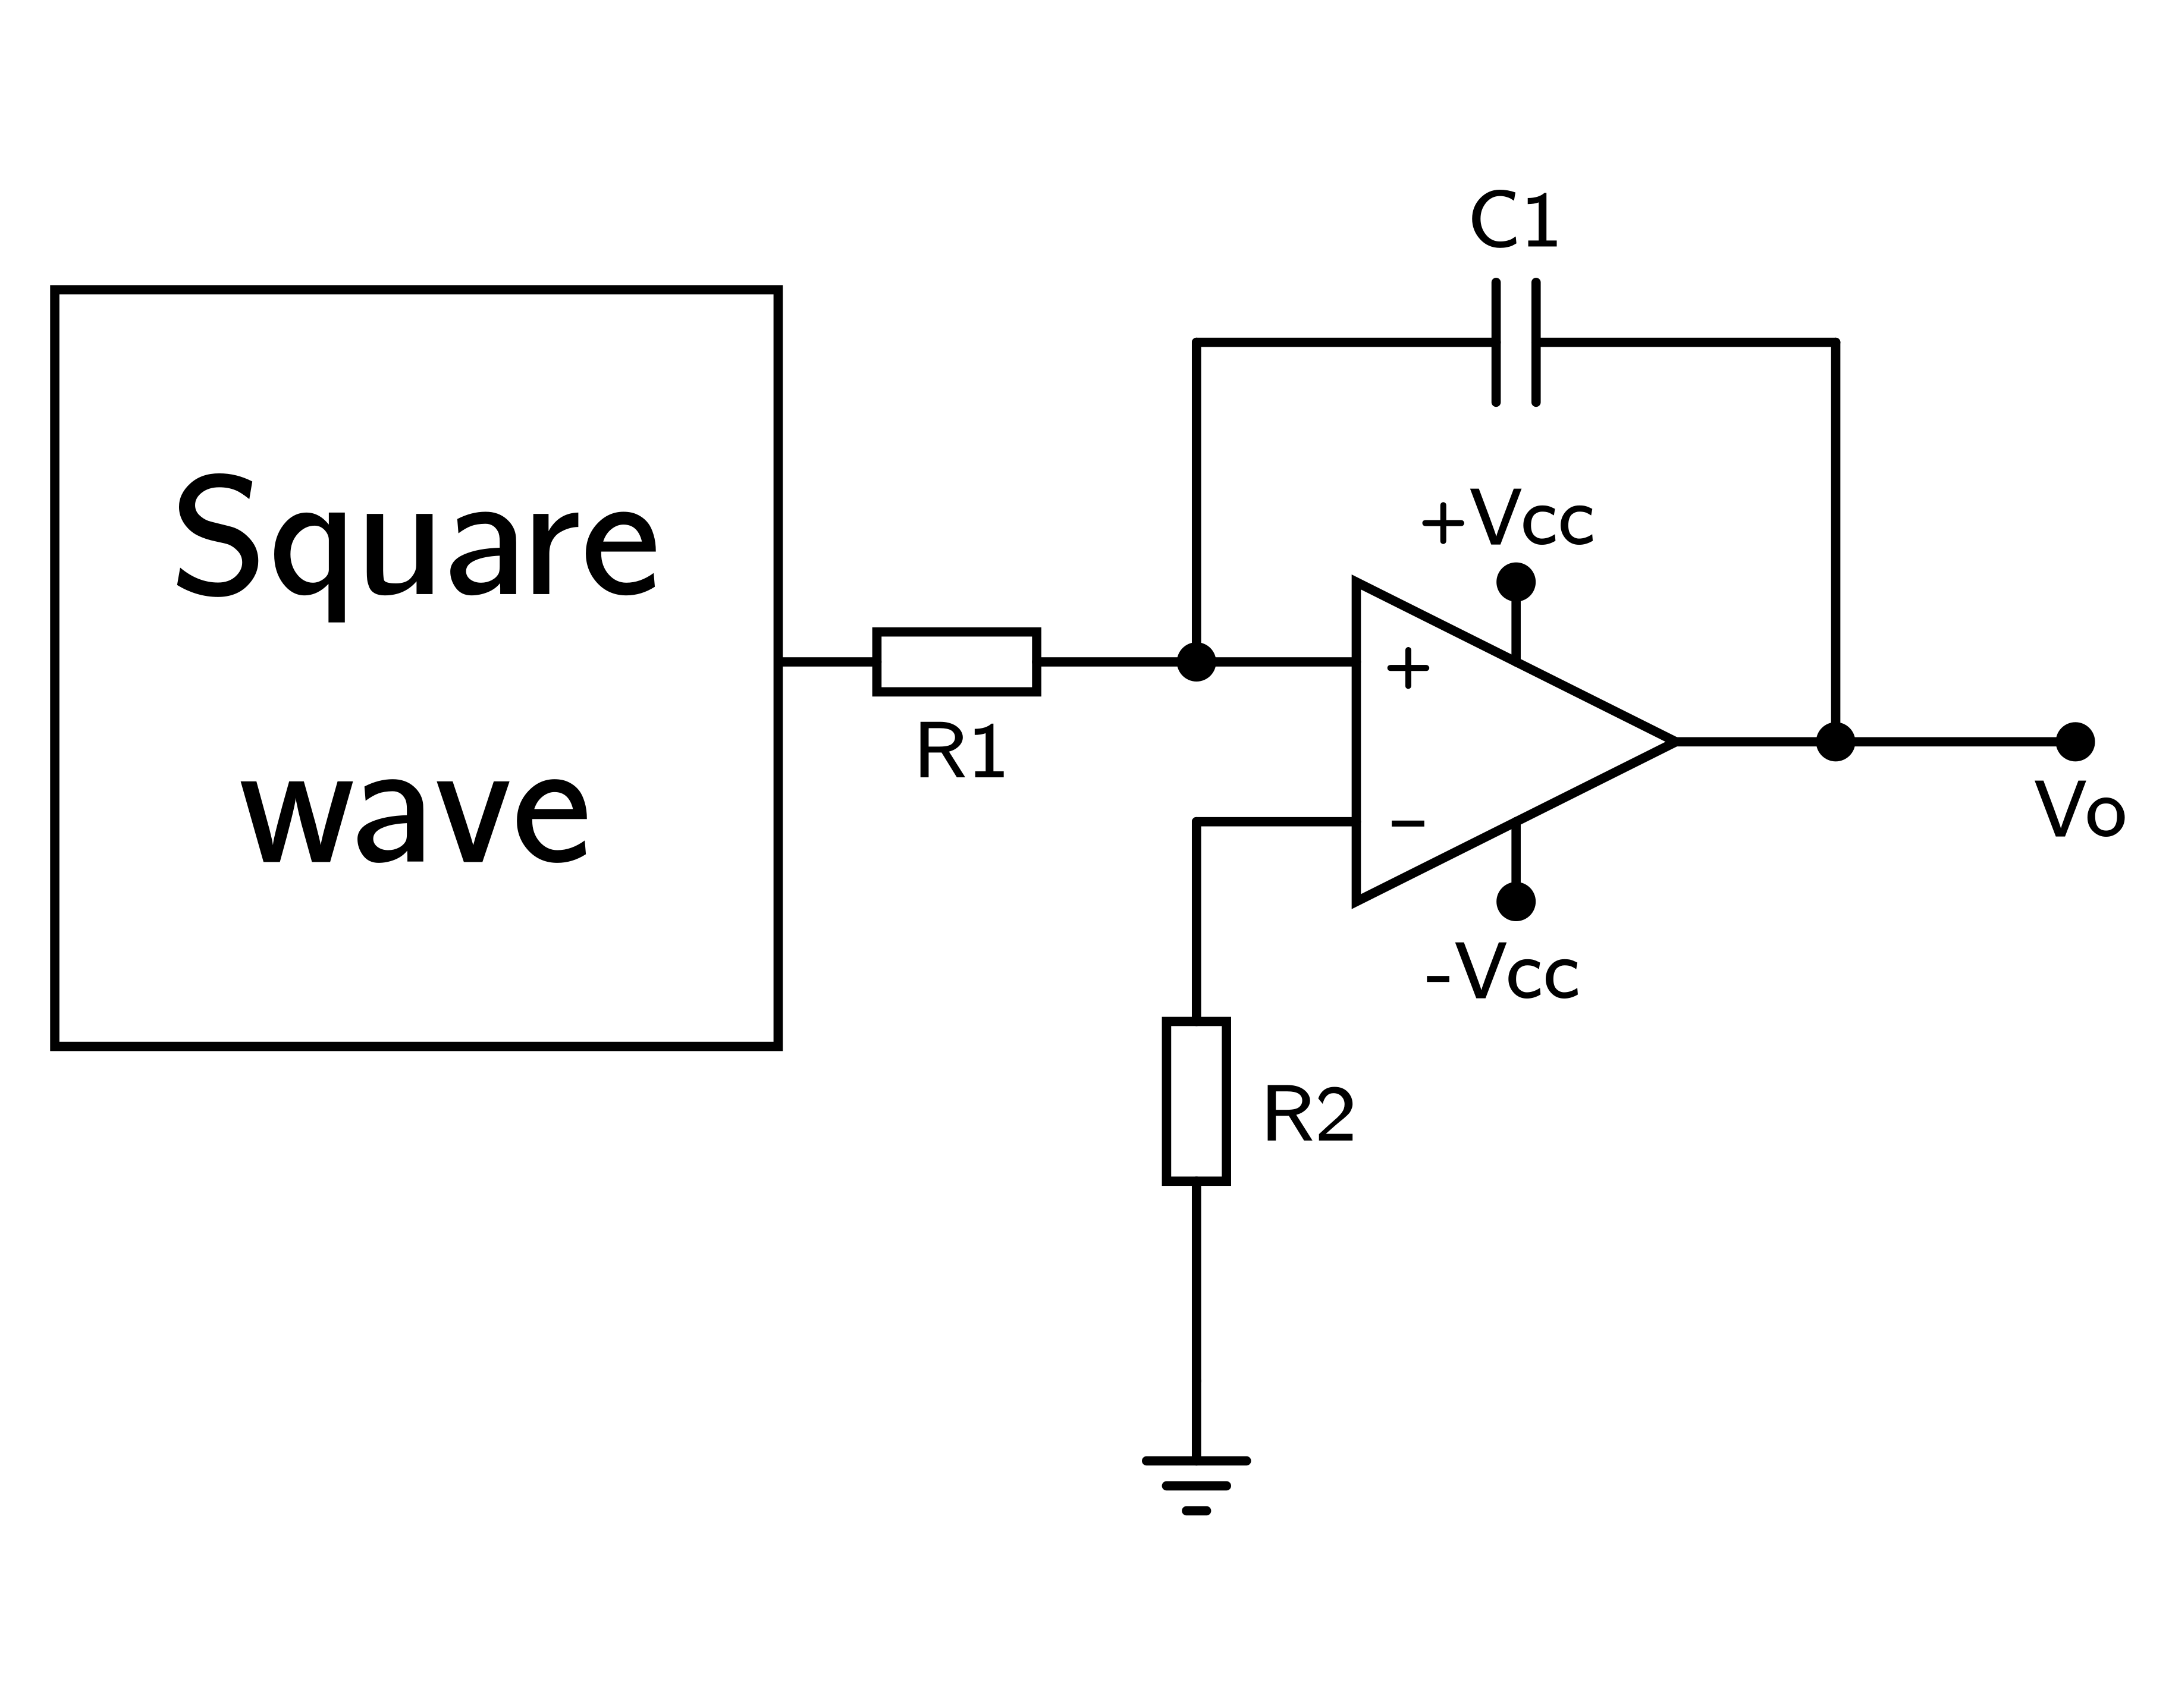
\includegraphics[width=0.7 \textwidth]{imgs/triang.png}
\caption{\label{fig:org66d79b1}integrator circuit with square wave as input}
\end{figure}


Here, \(R_{4}\) have to be \(10R_{3}\). Frequency is give by same relation as block 2.



\begin{figure}[htbp]
\centering
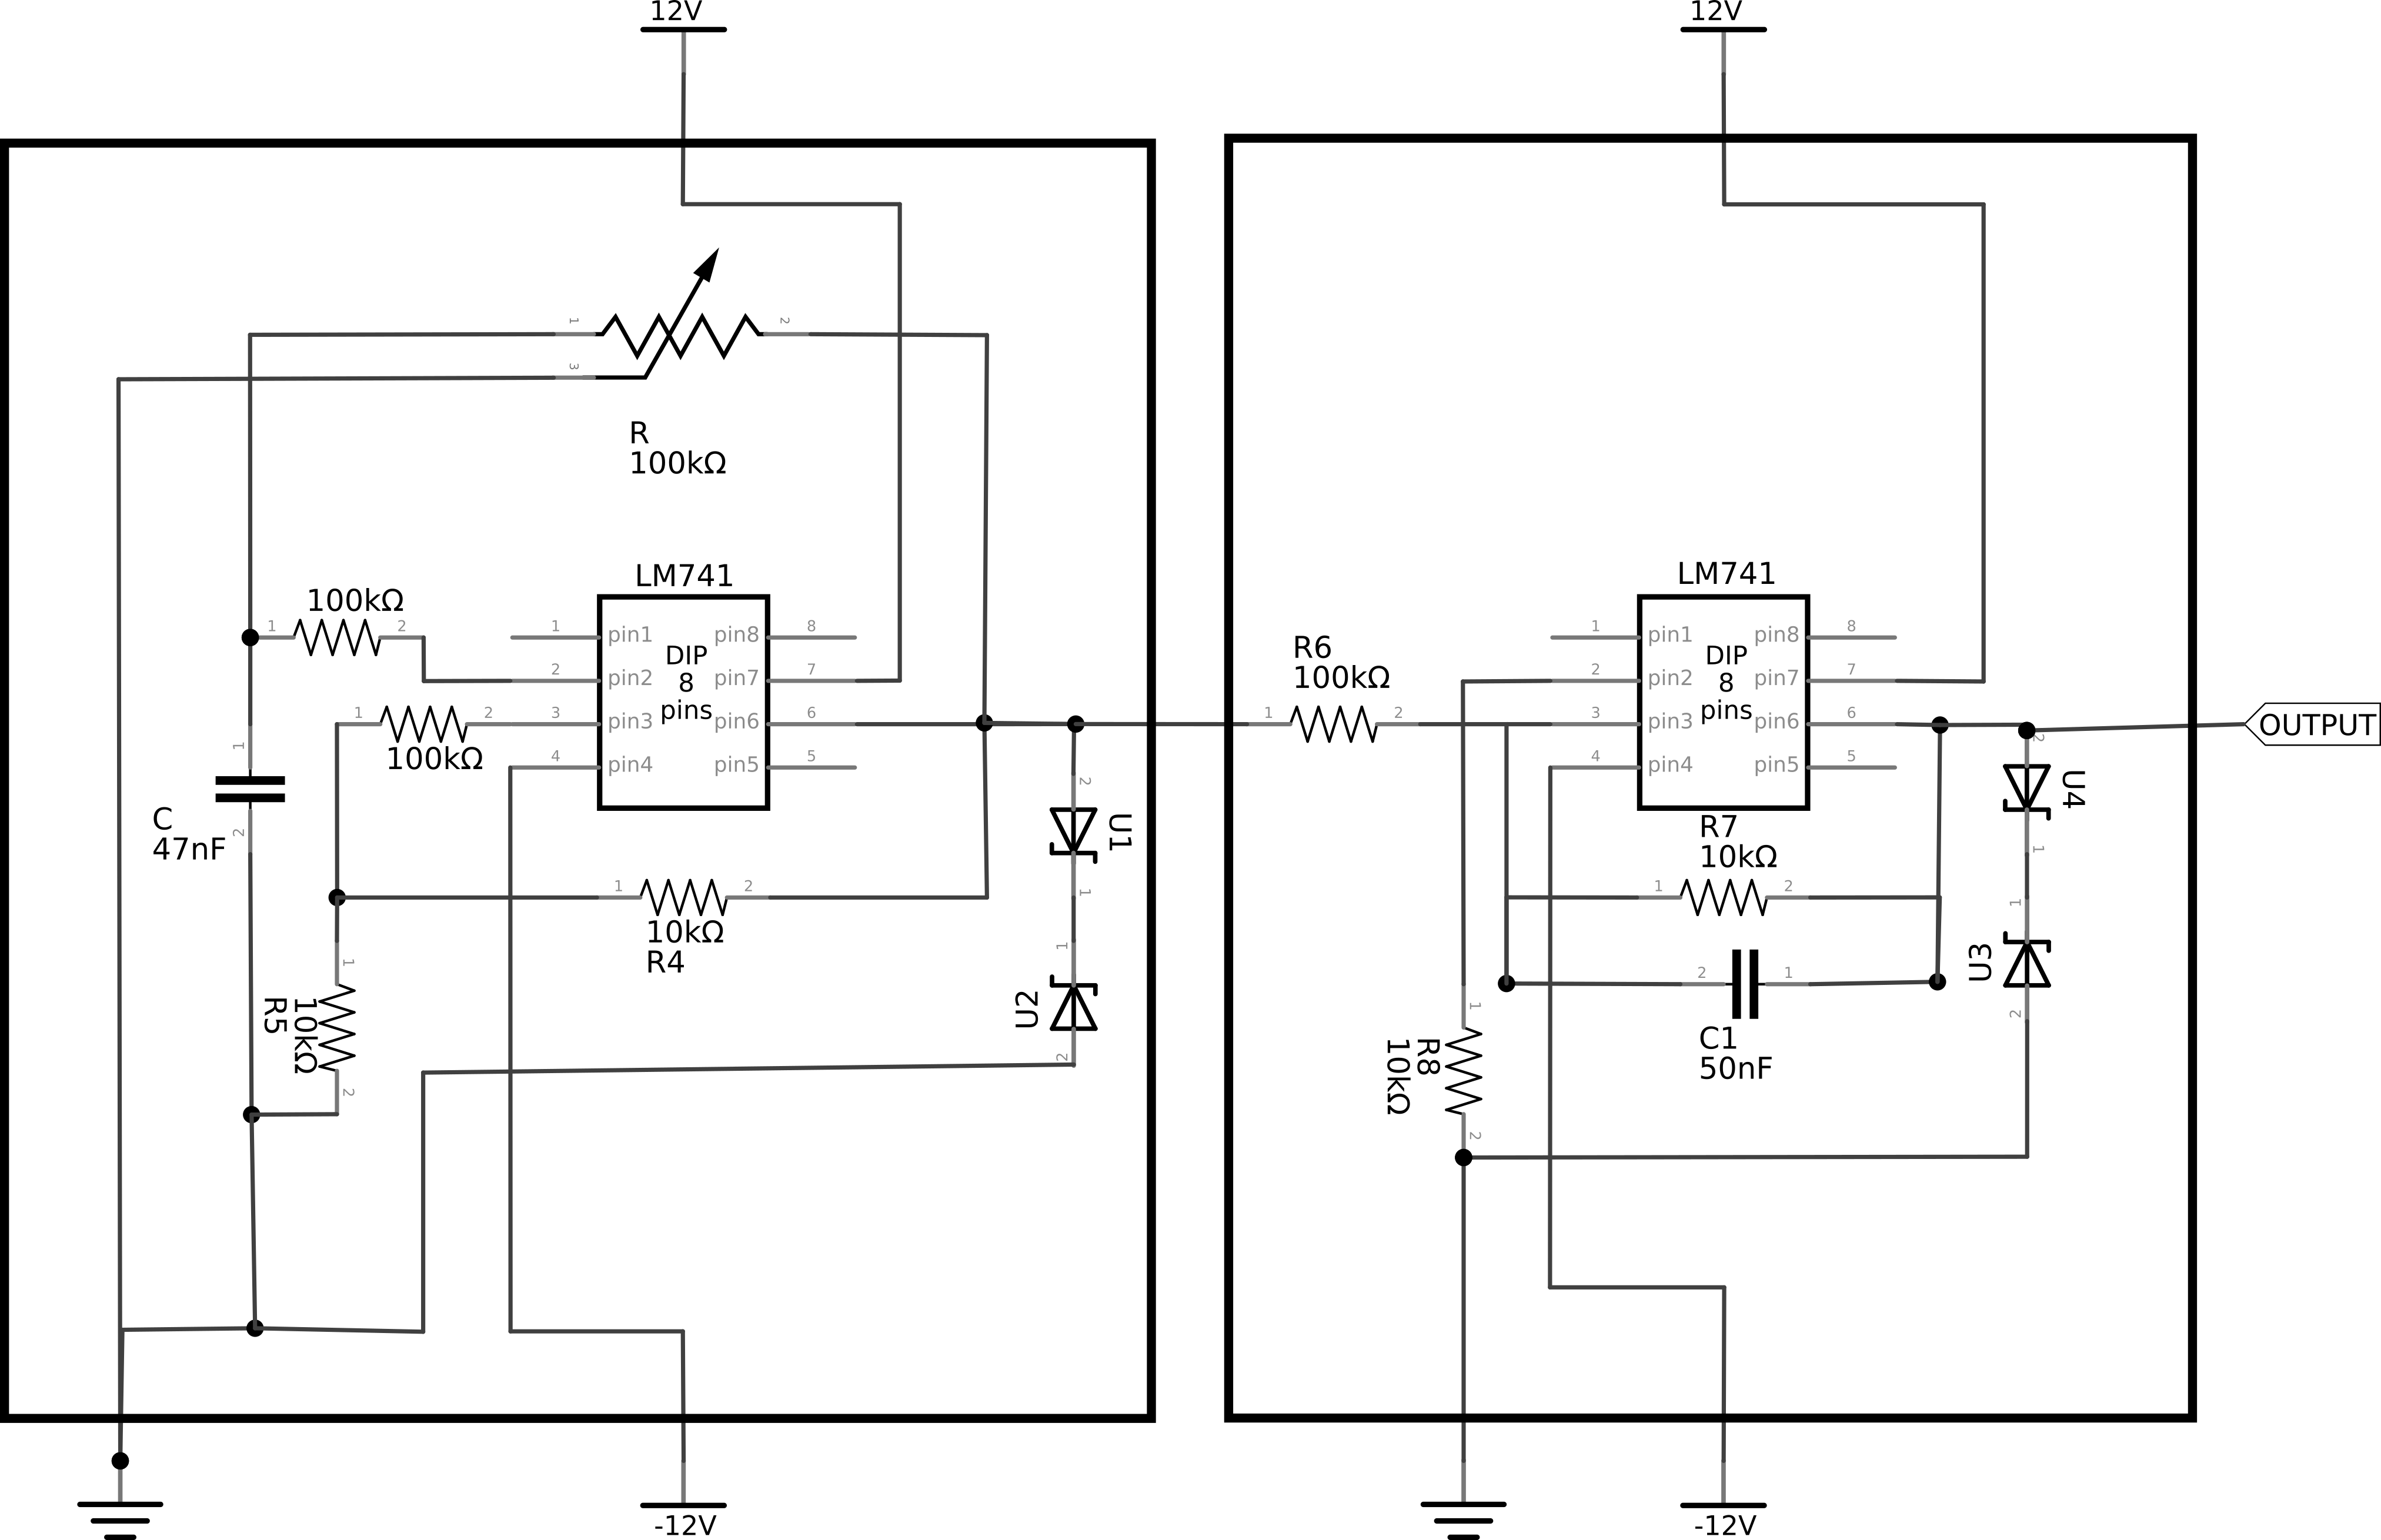
\includegraphics[width=0.95 \textwidth]{imgs/triangreal.png}
\caption{\label{fig:orgc55386a}block 3: triangluar wave generator}
\end{figure}




\section{connection and switching}
\label{sec:org3609da7}

For connection of all this block we have used push pull button with two poles. One for power controlling and other for output controlling. Basic diagram of this switch is drawn in figure.
\end{document}
